%
% section 50
%
\section*{Εισαγωγή στα Δίκτυα Ευρείας Περιοχής}

Τα τοπικά δίκτυα αποτελούν πολύ καλή λύση για επικοινωνία όταν η απόσταση που χρειάζεται να καλυφθεί είναι μικρή. Για μεγαλύτερες γεωγραφικές εκτάσεις αναπτύσσονται τα δίκτυα ευρείας περιοχής (WAN, Wide Area Networks). Η επέκταση των τοπικών δικτύων σε δίκτυα ευρείας περιοχής επιτυγχάνεται χρησιμοποιώντας κατάλληλες γραμμές σύνδεσης και δικτυακά εξαρτήματα όπως modems, γέφυρες, δρομολογητές κ.α.

\begin{figure}[!ht]
  \centering
  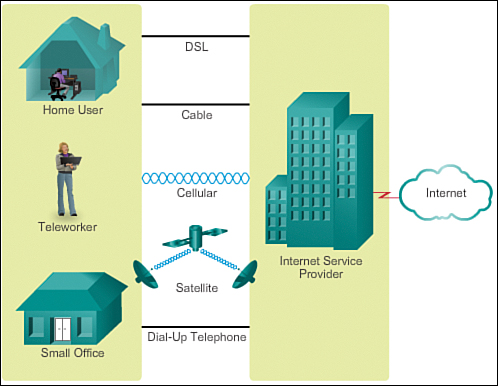
\includegraphics[width=0.95\textwidth]{images/chapter5/5-1}
  \caption {\textsl{Επιλογές Σύνδεσης σε WAN}}
  \label{5-1}
\end{figure} 

Για την ανάπτυξη γραμμών WAN μπορεί να χρησιμοποιούνται δίκτυα μεταγωγής (κυκλώματος ή πακέτου), δορυφορικές συνδέσεις, μικροκυματικές ζεύξεις, οπτικές ίνες ή σύστημα καλωδιακής τηλεόρασης.

Όσο αφορά το χρήστη, το δίκτυο ευρείας περιοχής φαίνεται να λειτουργεί με τον ίδιο ακριβώς τρόπο με το LAN. Αν το WAN έχει υλοποιηθεί με σωστές τεχνικές, δεν έχει καμιά διαφορά στη συμπεριφορά με το LAN (είναι όπως λέμε \emph{διάφανο}).

Είναι αρκετά δύσκολο για μια εταιρεία να εγκαταστήσει και να διαχειριστεί τις δικές της γραμμές WAN. Συνήθως τις νοικιάζει από κάποιο τηλεπικοινωνιακό φορέα ο οποίος διαθέτει συνήθως ήδη τις γραμμές και τον απαραίτητο εξοπλισμό. Οι τεχνολογίες που χρησιμοποιούνται στις υπηρεσίες δικτύων ευρείας περιοχής είναι:

\begin{itemize}
\item Επιλεγόμενες τηλεφωνικές γραμμές (κοινό τηλεφωνικό δίκτυο)
\item Μόνιμες ή μισθωμένες γραμμές
\item Πρότυπο X.25
\item Πρότυπο Frame Relay
\item Γραμμές ISDN
\item ATM (Asychronous Transfer Mode, Ασύγχρονος Τρόπος Μεταφοράς)
\item Γραμμές xDSL
\item Τεχνολογίες FTTH (Fiber To The Home, Οπτική Ίνα για Οικιακή Χρήση) και Metro Ethernet (Μητροπολιτικό δίκτυο βασισμένο σε τεχνολογία Ethernet)
\item Ασύρματες και Δορυφορικές ζεύξεις
\end{itemize}

Από τις παραπάνω τεχνολογίες, η X.25 και Frame Relay έχουν ουσιαστικά ήδη καταργηθεί.